\subsubsection{Validación del sistema de trituración}

Para validar el componente seleccionado, se verificó el tamaño de las partículas a la entrada y a la salida, teniendo a la entrada del sistema una abertura ovalada de un diámetro mínimo de 5 centímetros, por lo que a la entrada del sistema se puede insertar la materia orgánica a procesar sin ningún tipo de problema.

A la salida se encuentra un disco ranurado , cual puede ser cambiado de acuerdo a nuestras necesidades, el molino de carne ya viene con un disco ranurado con orificios de 5mm de diámetro, lo cual permite obtener a materia orgánica lista para su procesamiento con una dimensión menor a la máxima permitida. 

\begin{figure}[h]
            \centering
            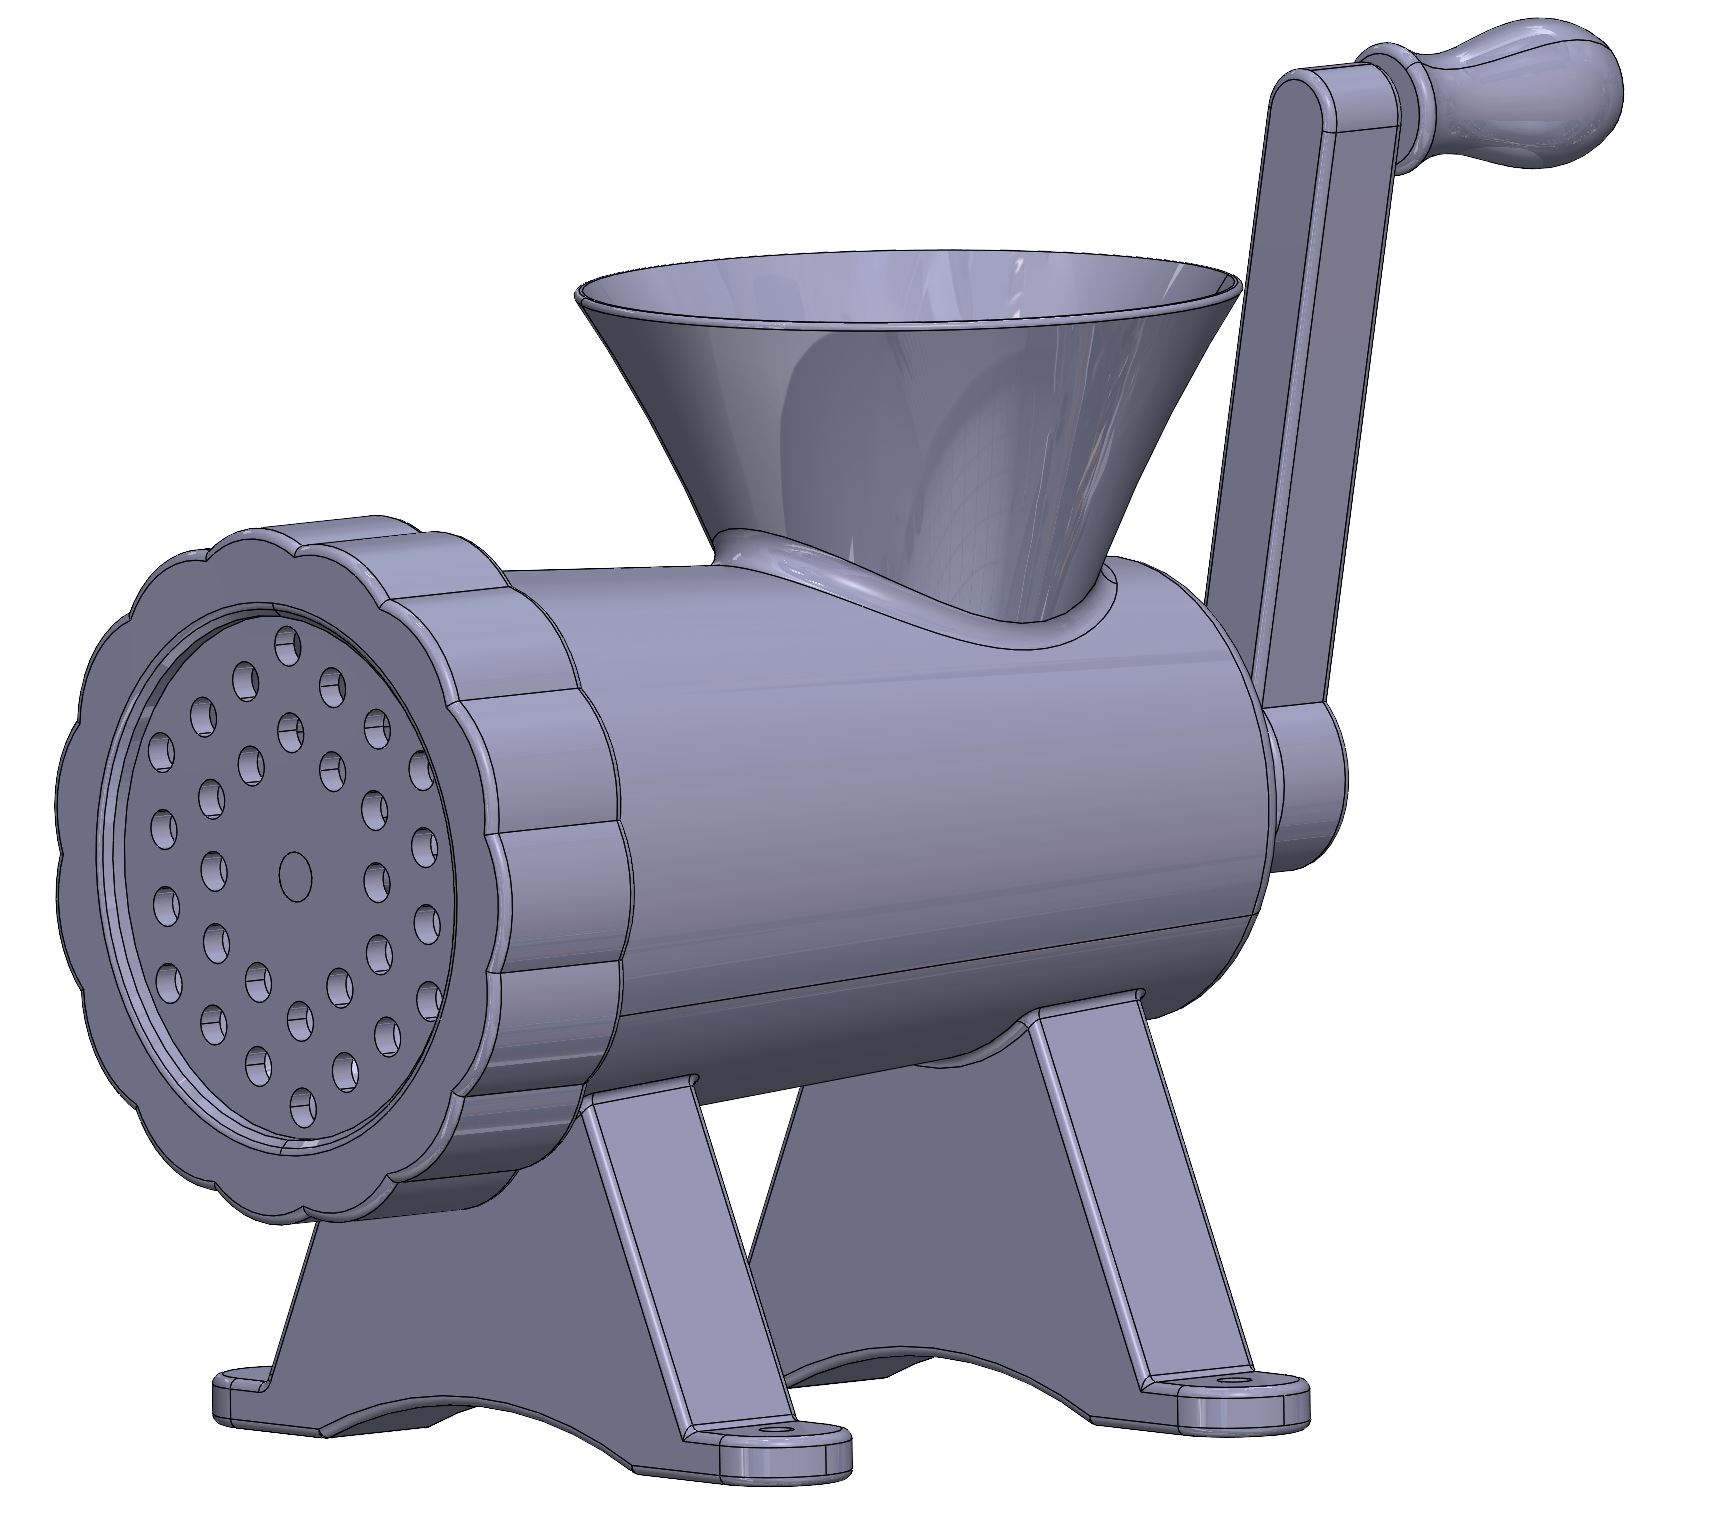
\includegraphics[scale=0.3]{images/Capitulo 4/S4/Modelo-CAD-triturador.png}
            \caption{Modelo CAD del molino de carne manual}
            \label{fg:molinoCAD}
\end{figure}

El molino consiste en un disco helicoidal de paso variable encargado de ir presionando la materia orgánica hacia el disco ranurado, en el eje va montada una cuchilla que ayuda a cortar la materia orgánica en trozos pequeños que puedan fácilmente salir por las ranuras del disco.